\chapter{Interactive Light Source}
\label{sec:lamp}

The previously mentioned light source for the scenario is built around a 12 V powered RGB \ac{LED} strip, which can be purchased for home lighting or car decoration. It is approximately XX cm long and features XX \ac{LED}s on each XX cm long segment. The original controller box which included an \ac{IR} receiver for a remote was removed and replaced by an Arduino Uno \cite{arduino_uno} with a custom shield. 

The shield features a Roving Networks RN42 Bluetooth module \cite{datasheet_rn42} and some transistors for upscaling the voltage from 3.5 V to 12 V. The whole setup is powered by a standard 12 V power supply and encased in a spherical lamp shade made from translucent glass in order to diffuse the spotted impression of the LED strip (cf. figure \ref{fig:lamp}).

\begin{figure}[bth]
	\begin{center}
		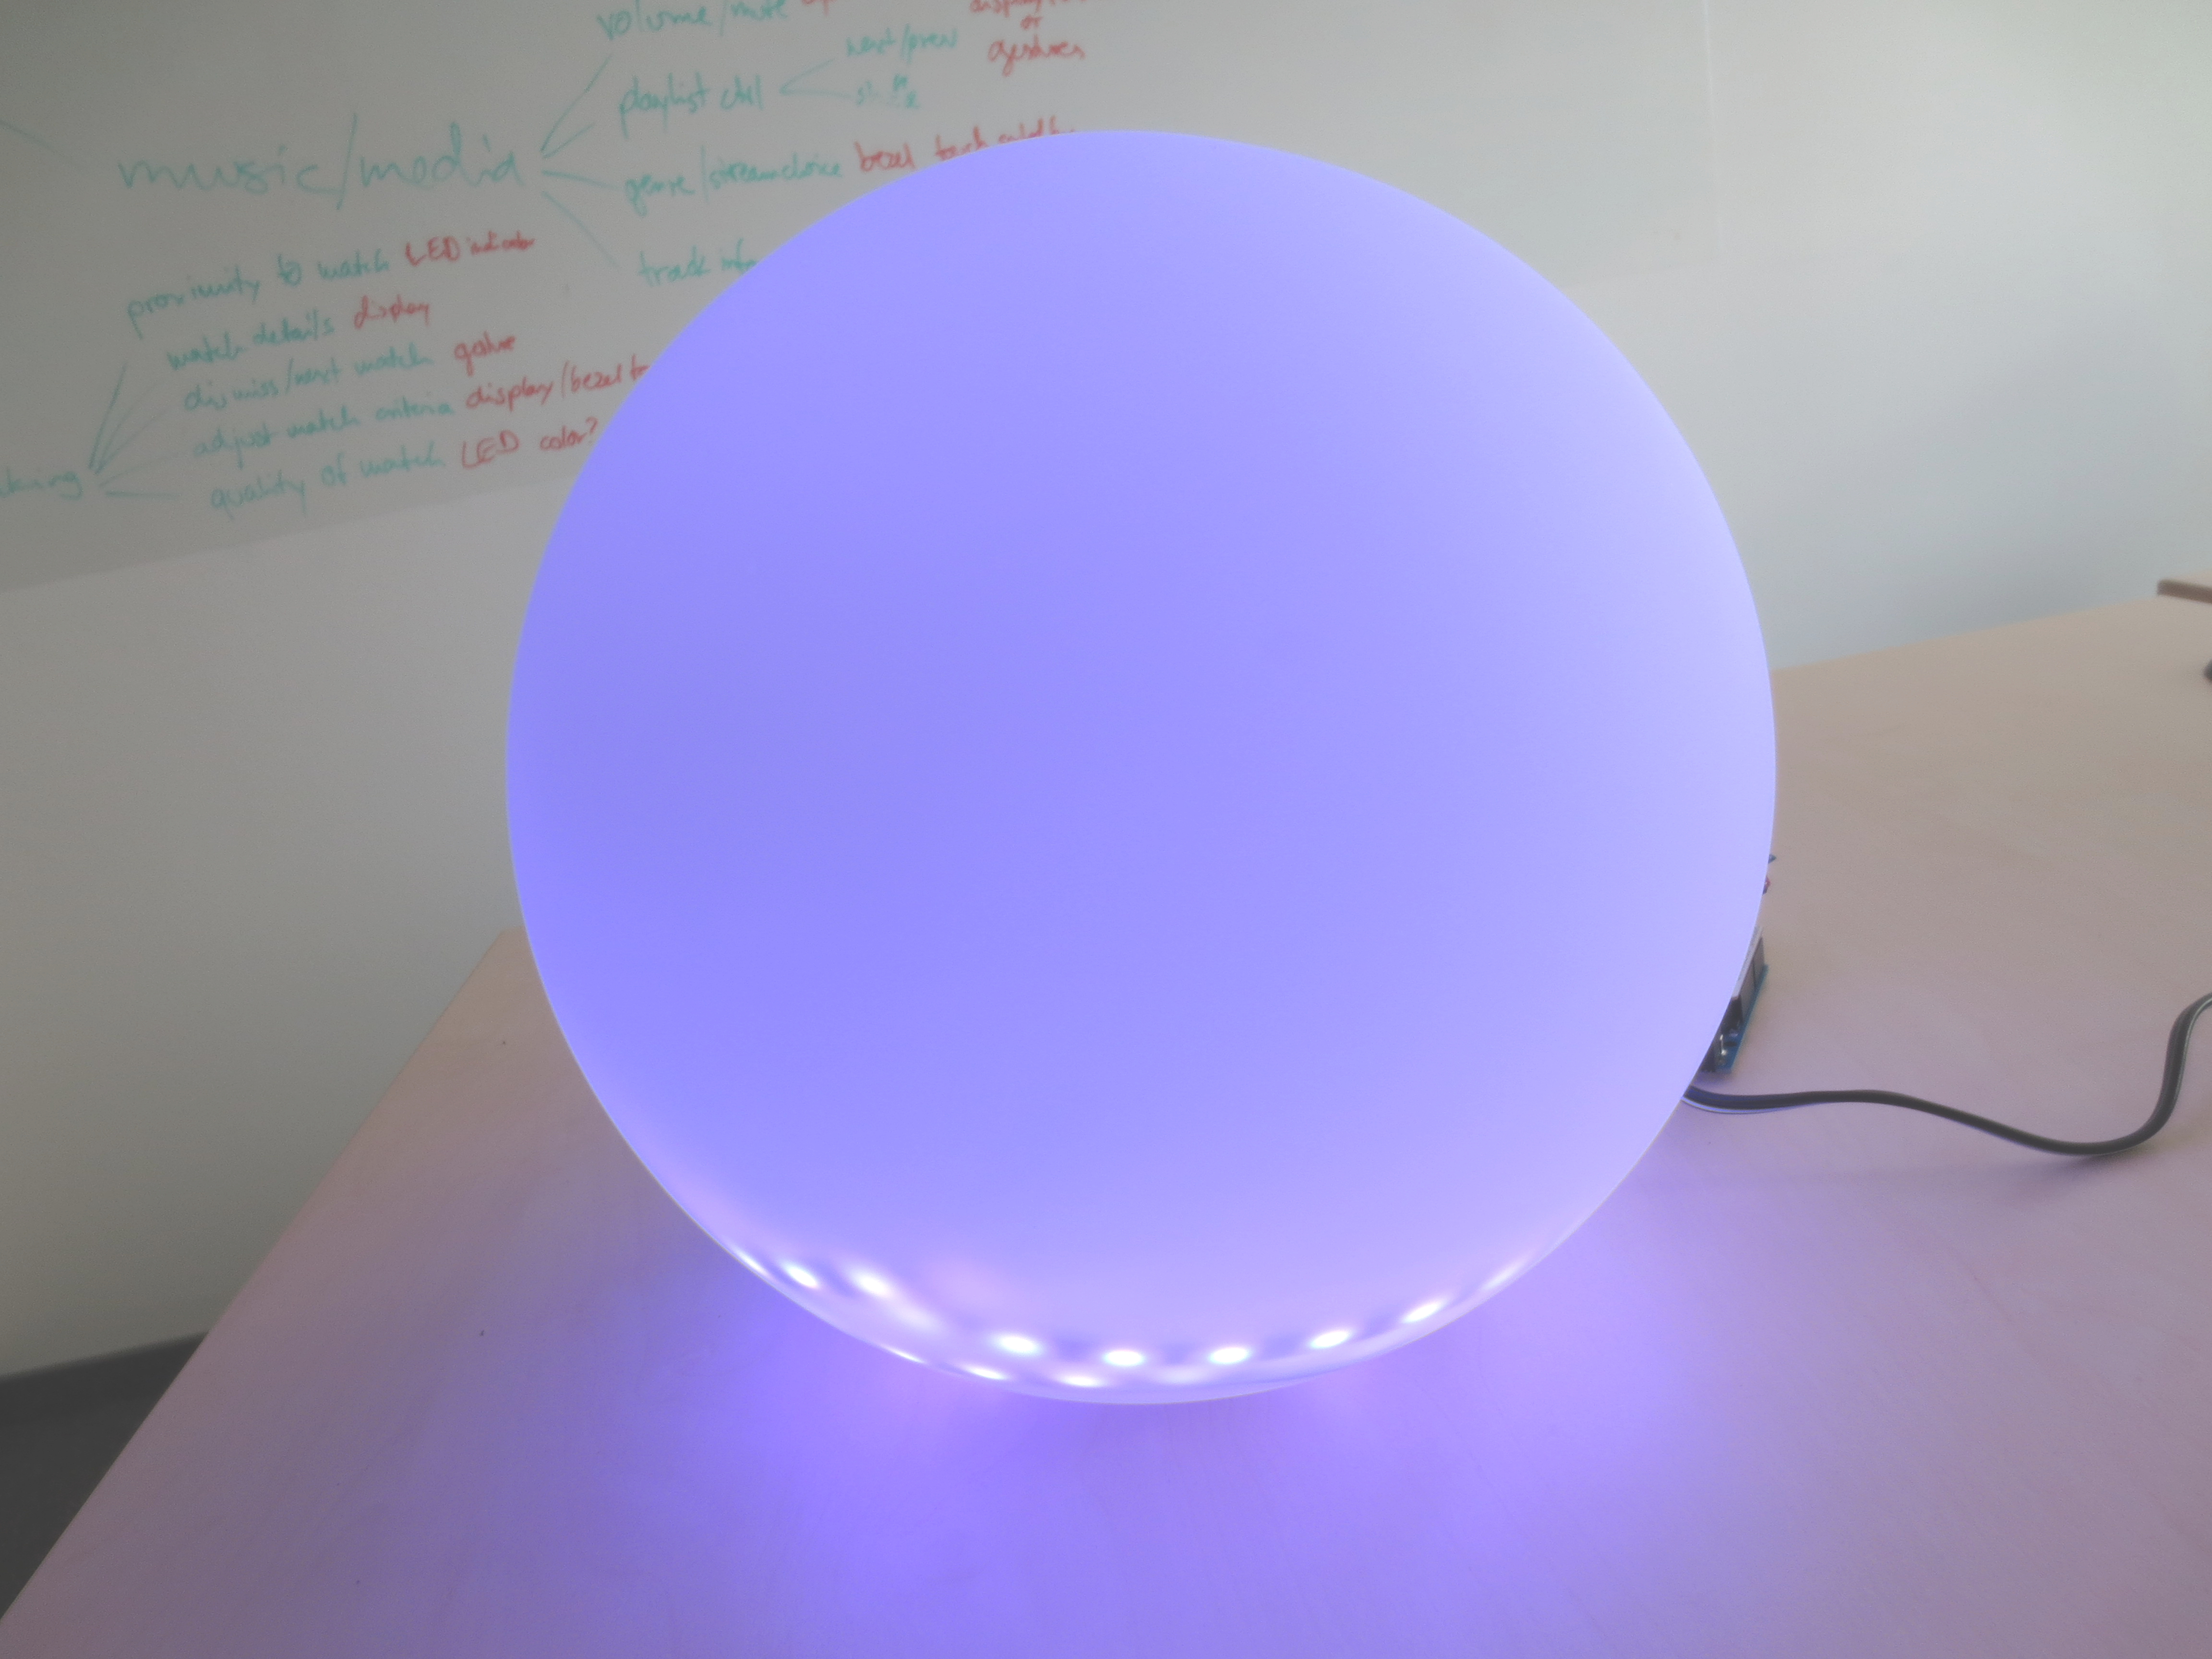
\includegraphics[width=.5\linewidth]{gfx/lamp.png}
	\end{center}
	\label{fig:lamp}
	\caption{The interactive light source, encased.}
\end{figure} 

Communication with the bracelet takes place via Bluetooth. The RN42 module implements the Bluetooth \ac{SPP} and can be accessed easily with the \texttt{SoftwareSerial} module from the Arduino standard library. The lamp is configured as a Bluetooth slave, the bracelet acts as the master device. For command transmission, a serial connection is established over the Bluetooth link between the devices. Once it is set up, the master transmits a nine-digit string composed from three values from $000$ to $255$. Note that all values must have three digits, leading zeros must not be omitted. These values represent the intensities of the red, green, and blue channel respectively. The algorithm on the Arduino feeds them into the platform's analog outputs which feature \ac{PWM}. These output signals are scaled as mentioned before and so the light color changes. A simple fading algorithm prevents disruptive flashing while switching colors.

It turned out that the RGB \ac{LED}s use a lot of current, a test with an adjustable power supply yielded that the lights become much brighter with increased current. The power supply was limited to XX Ampere and there was no saturation in bightness indicated at this level. However, the standard power supply mentioned above serves only XX A which results in less brightness. A way to improve this would be to shorten the \ac{LED} strip by cutting off several segments.